\documentclass[11pt]{article}
\usepackage{graphicx}    % needed for including graphics e.g. EPS, PS
\topmargin -1.5cm        % read Lamport p.163
\oddsidemargin -0.04cm   % read Lamport p.163
\evensidemargin -0.04cm  % same as oddsidemargin but for left-hand pages
\textwidth 16.59cm
\textheight 21.94cm 
%\pagestyle{empty}       % Uncomment if don't want page numbers
\parskip 7.2pt           % sets spacing between paragraphs
%\renewcommand{\baselinestretch}{1.5} % Uncomment for 1.5 spacing between lines
\usepackage{amsmath}
\usepackage{amsfonts}
\usepackage{amsthm}
\usepackage{verbatim}
\usepackage{subfigure}
\usepackage{cite}
\parindent 0pt		 % sets leading space for paragraphs
\author{Fermi Ma \and Erik Waingarten}
\title{Data Structures Final Project:\\
A Linear Programming Approach to Dynamic Optimality}

\newtheorem{theorem}{Theorem}
\newtheorem{lemma}[theorem]{Lemma}
\newtheorem{observation}{Observation}

\begin{document}         
\maketitle

\section{Introduction}

We consider the the points in the plane problem. The problem is defined as follows:

\vbox{
\noindent
\begin{quote}
Given a set $P$ of $n$ points $(x_i,y_i)$ in the $xy$ plane, no two on a common row or column, find the minimal point set $Q \supseteq P$ such that for any two points in $Q$ not on a common row or column, the rectangle they span contains another point in $Q$.
\end{quote}
}

Point sets $Q$ that satisfy the condition that any two points in $Q$ that span a rectangle contain another point in $Q$ are referred to as \emph{arborally satisfied} point sets.

It is natural to restrict attention to the grid of intersection points ``induced" by the set of points $P$: extend horizontal and vertical lines through each point in $P$ and consider only the $O(n^2)$ intersections of these lines. It is easy to show that in any arborally satisfied point set $P$, points that are not grid intersections can be moved to positions that are. An example of such a grid is given Figure~\ref{fig:instance}.

\begin{figure}
\centering
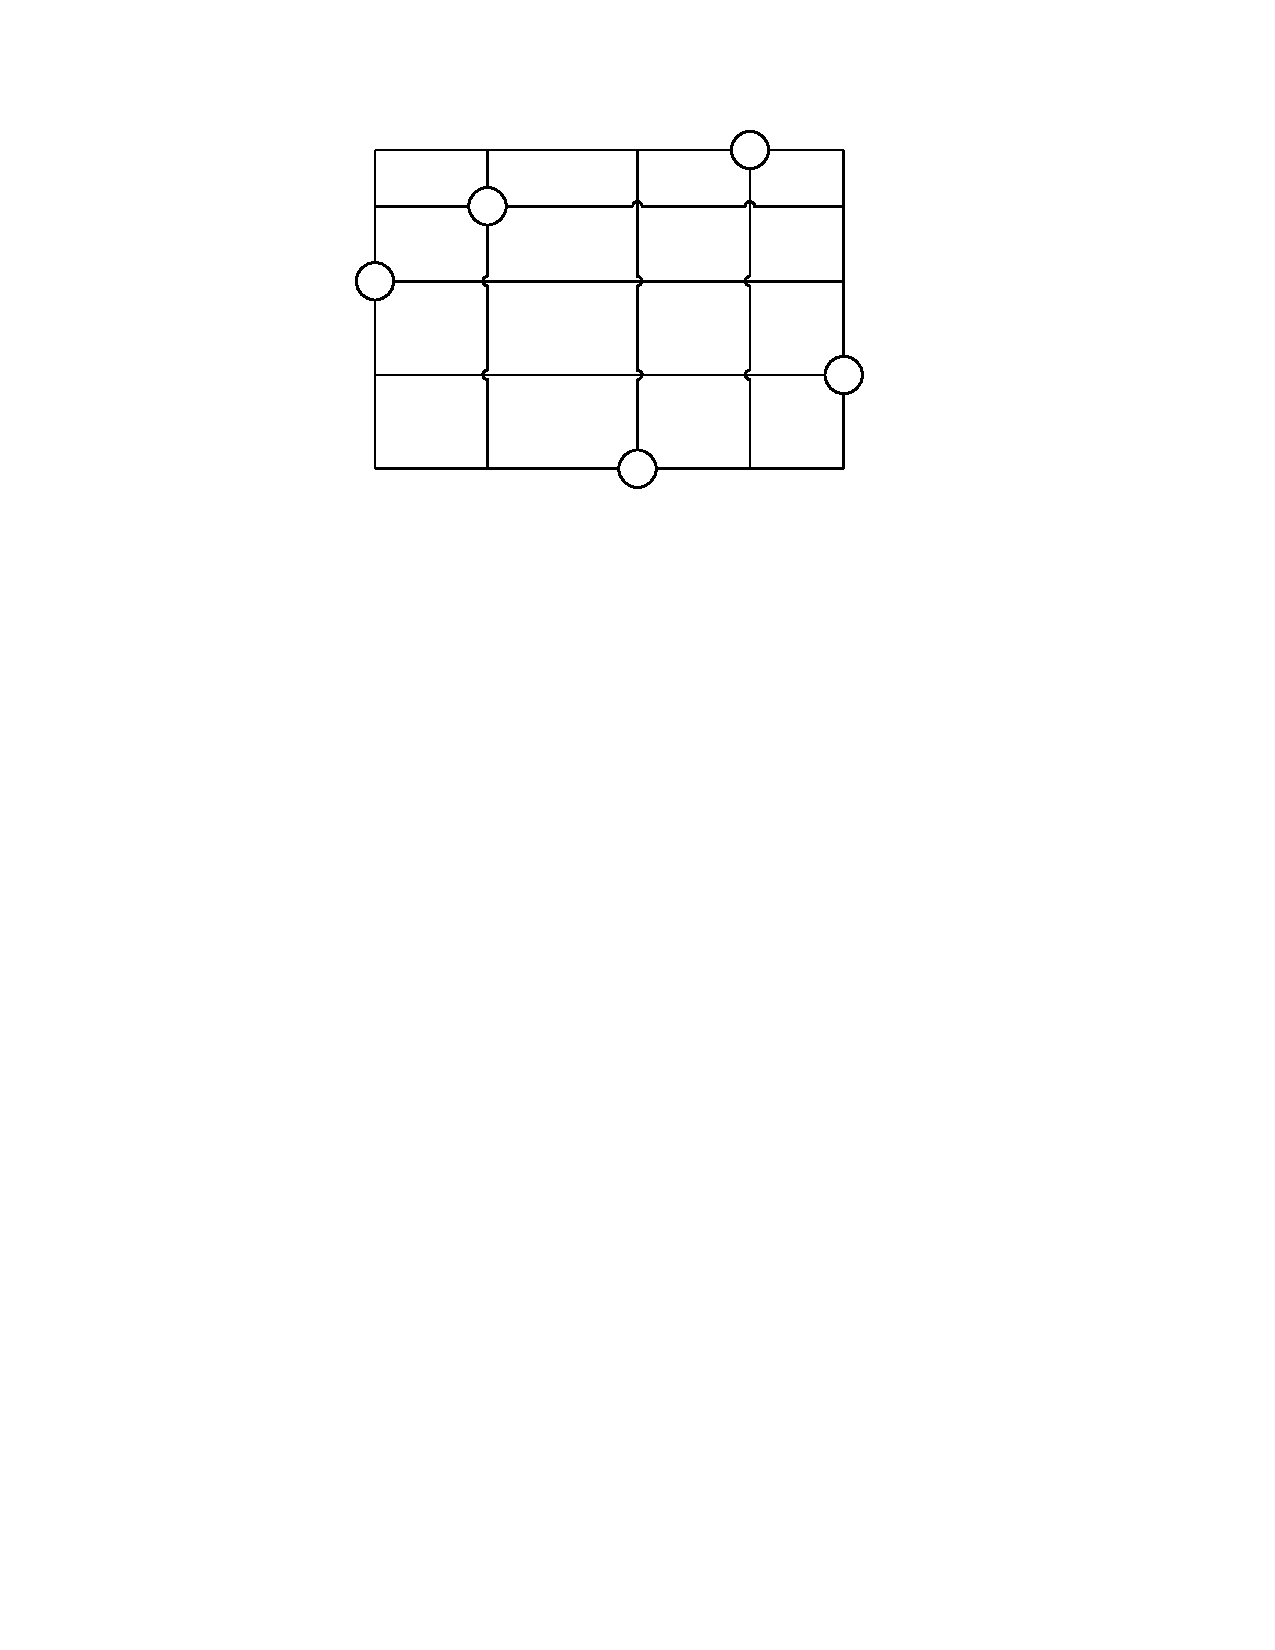
\includegraphics[width=0.3\linewidth]{instance.pdf}
\caption{Instance of points in the plane}
\label{fig:instance}
\end{figure}

We can directly correspond an integer linear program (ILP) to the problem by assigning an indicator variable to each grid point, where the variable is set to 1 if the point is included and is 0 otherwise. This gives the obvious objective of minimizing the sum of all the variables, and leaves the task of writing down the arboral satisfaction property in terms linear constraints. While other linear programming approaches may exist, this setup feels the most natural and so we restrict our attention to it.

We found that it was possible to write down an exact ILP with $O(n^2)$ constraints of size $O(n^2)$, and another ILP with $O(n^2)$ constraints of size $O(n)$ with the same optimal solutions to the original problem. We attempted to use the second ILP formulation to generate an approximation algorithm for the problem by considering the relaxed linear program, but methods such as viewing the problem as a max flow problem and taking the dual proved unsuccessful. Our experiments indicated that the ILP had an integrality gap strictly greater than 1, and we were later able to demonstrate an unbounded integrality gap for the specific ILP we had written down. This indicates that common approximation algorithm for that specific ILP will not work, and we conjecture that an unbounded integrality gap exists for any ILP formulation of the problem. We were not able to prove the conjecture, but we provide some useful observations.

\section{Bounds on the Problem}

Observe that $|Q| = \Omega(n)$ since $P \subset Q$. Furthermore, $|Q| = O(n^2)$ is trivially true since every grid intersection point can be included (see Figure~\ref{fig:instance}). However, there exists a stronger bound (communicated to us verablly by Erik Demaine):

\begin{theorem} $|Q| = O(n\log(n))$
\end{theorem}
\begin{proof}
Let $m$ be the median in the $x$ axis of $P$, this divides $P$ into two sets of size $O(\frac{n}{2})$. Now for each $(x,y) \in P$, let $(m, y) \in Q$. Then recursively solve both subsets of size $O(\frac{n}{2})$. Note that for every two points, they will be divided by the recursion at some point. This means that there is a point in the rectangle. This gives the recursion $|Q| = T(n) = 2T(\frac{n}{2}) + O(n)$, therefore, $|Q| = O(n \log n)$. 
\end{proof}

The same bound arises from viewing each arborally satisfied set as an access sequence of a binary search tree algorithm. \cite{geometryBST}

\section{A First Attempt}

We set up the indicator variables as explained in the introduction, labeling them as $b_{jk}$, where $j$ and $k$ are labels on the grid intersection points (labelled so that $b_{00}$ is the lower left grid point, $b_{01}$ is the point directly above, and $b_{10}$ is the point directly to the right).

Consider the following set of constraints:

\begin{align}
2b_{ij} + 2b_{nm} - \left(\sum_{i \leq k \leq n}\sum_{j\leq l \leq m} b_{kl}\right) &\leq 1  \hspace{.3in} \forall i<n, j<m \\
2b_{im} + 2b_{nj} - \left(\sum_{i \leq k \leq n}\sum_{j\leq l \leq m} b_{kl}\right)  &\leq 1  \hspace{.3in} \forall i<n, m<j
\end{align}

We claim that these constraints exactly capture arboral satisfaction. Constraints of type (1) correspond to all possible ``positive" rectangles, and constraints of type (2) correspond to all possible ``negative" rectangles.

To see the equivalence, first consider constraints of type (1). If points in the grid corresponding to $b_{ij}$ and $b_{nm}$ are present, the rectangle they span must be satisfied by some point corresponding to $b_{kl}$ such that   $i\leq k \leq n$ and $j \leq l \leq m$ (although it cannot equal to $b_{ij}$ or $b_{nm}$). The constraint ensures precisely this: if $b_{ij} = b_{nm} = 1$, at least one other $b_{kl}$ in the parenthesized term must be set to 1, or else the entire left hand side will be a quantity greater than 1. The constraints of type (2) work the same way.

\begin{comment}
An easy way to think of the constraints is that we are taking the sum of the points that create a rectangle minus every point inside that rectangle which is not the set points, and that this must be less than 1. This says that if both points of the corners are set to 1, then the sum will be 2, which means that there must be at least one point inside the rectangle set to 1. Thus the rectangle is satisfied. 
\end{comment}
If either of the corner vertices are not present, the rectangle corresponding to the constraint should be inactive, as there does not have to be a point satisfying it. Note that the constraint captures this behavior, since in this case the positive terms will be at most 1, satisfying the inequality no matter what the term in parenthesis is.

If we have such constraint for every possible rectangle, we will have an arborally satisfied set. Note that this integer linear program will solve for the exact optimal solution.

The primary issue with writing constraints of this form is this is that they are possibly quadratic in size, which makes it unlikely for them to yield useful approximation techniques. It turns out that we can simplify the constraints to be linear in size, as we show in Section~\ref{A Second Attempt: Reducing Constraint Size}, and this seems more promising since the dynamic optimality problem is focused on constant factor approximations. 

\section{A Second Attempt: Reducing Constraint Size}
\label{A Second Attempt: Reducing Constraint Size}

Any arborally satisfied point set has all the rectangles are satisfied by grid points that lie on their edges ~\cite{geometryBST}. This allows us to reduce the size of the constraints from $O(n^2)$ to $O(n)$.

We claim that the following set of constraints captures arboral satisfaction: 

\begin{align}
b_{ij} + b_{nm} - \left(\sum_{l=i+1}^{n-1} (b_{lj}+b_{lm}) + \sum_{l=j+1}^{m-1} (b_{il} + b_{nl}) + b_{im} + b_{nj} \right) &\leq& 1 & \hspace{.3in} \forall i<n, j<m \\
b_{im} + b_{nj} - \left(\sum_{l=i+1}^{n-1} (b_{lj}+b_{lm}) + \sum_{l=j+1}^{m-1} (b_{il} + b_{nl}) + b_{ij} + b_{nm} \right) &\leq& 1 & \hspace{.3in} \forall i<n, j<m
\end{align}

Constraints of type (3) correspond to all possible ``positive" rectangles, and constraints of type (4) correspond to all possible ``negative" rectangles. This captures arboral satisfaction for the same reason that the constraints of types (1) and (2) do. The only difference is that these constraints only look at vertices on the edges of rectangles. Figure~\ref{fig:rectangles} gives the graphical interpretation of the contraints, where he white circles are added  and the black circles are subtracted, the black lines correspond to all the points in between being subtracted.

\begin{figure}
\centering
\subfigure[Positive rectangle]{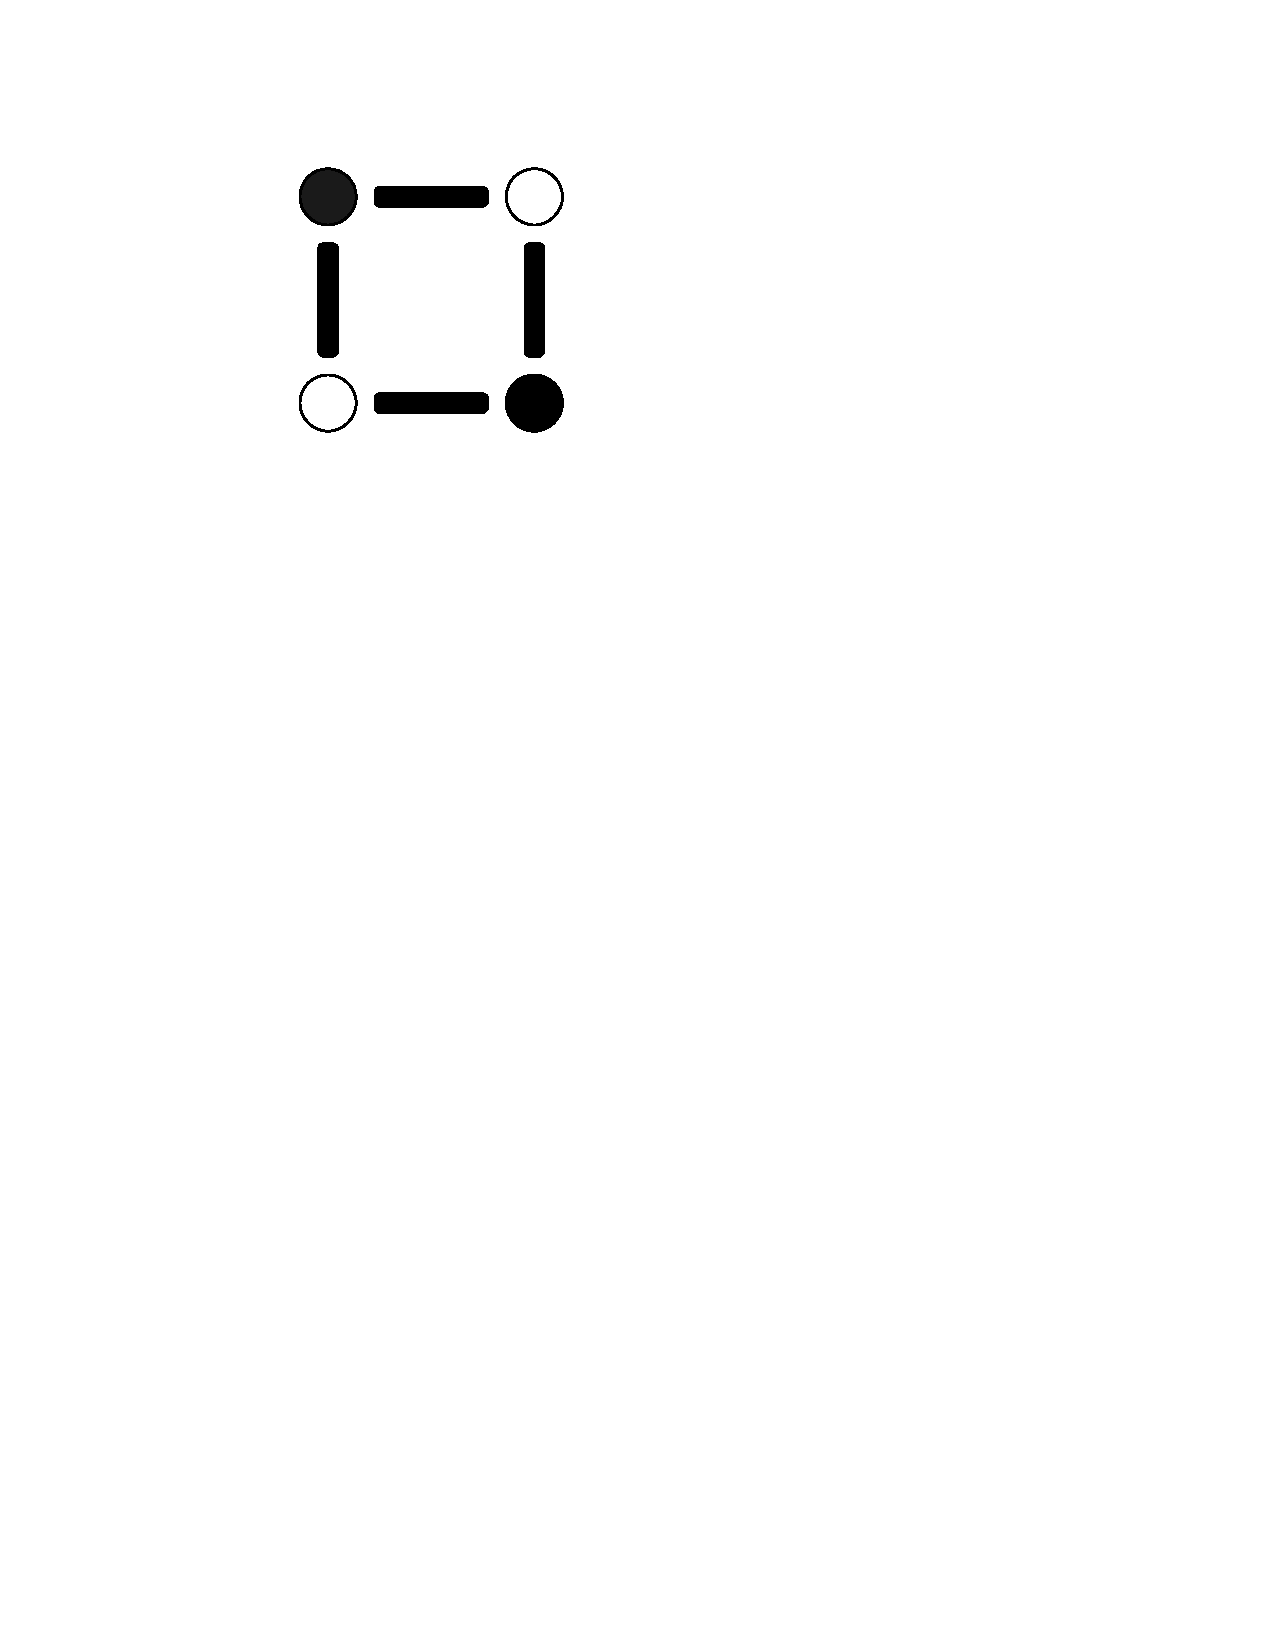
\includegraphics[width=0.2\linewidth]{positive.pdf}\label{fig:positive}}
\subfigure[Negative rectangle]{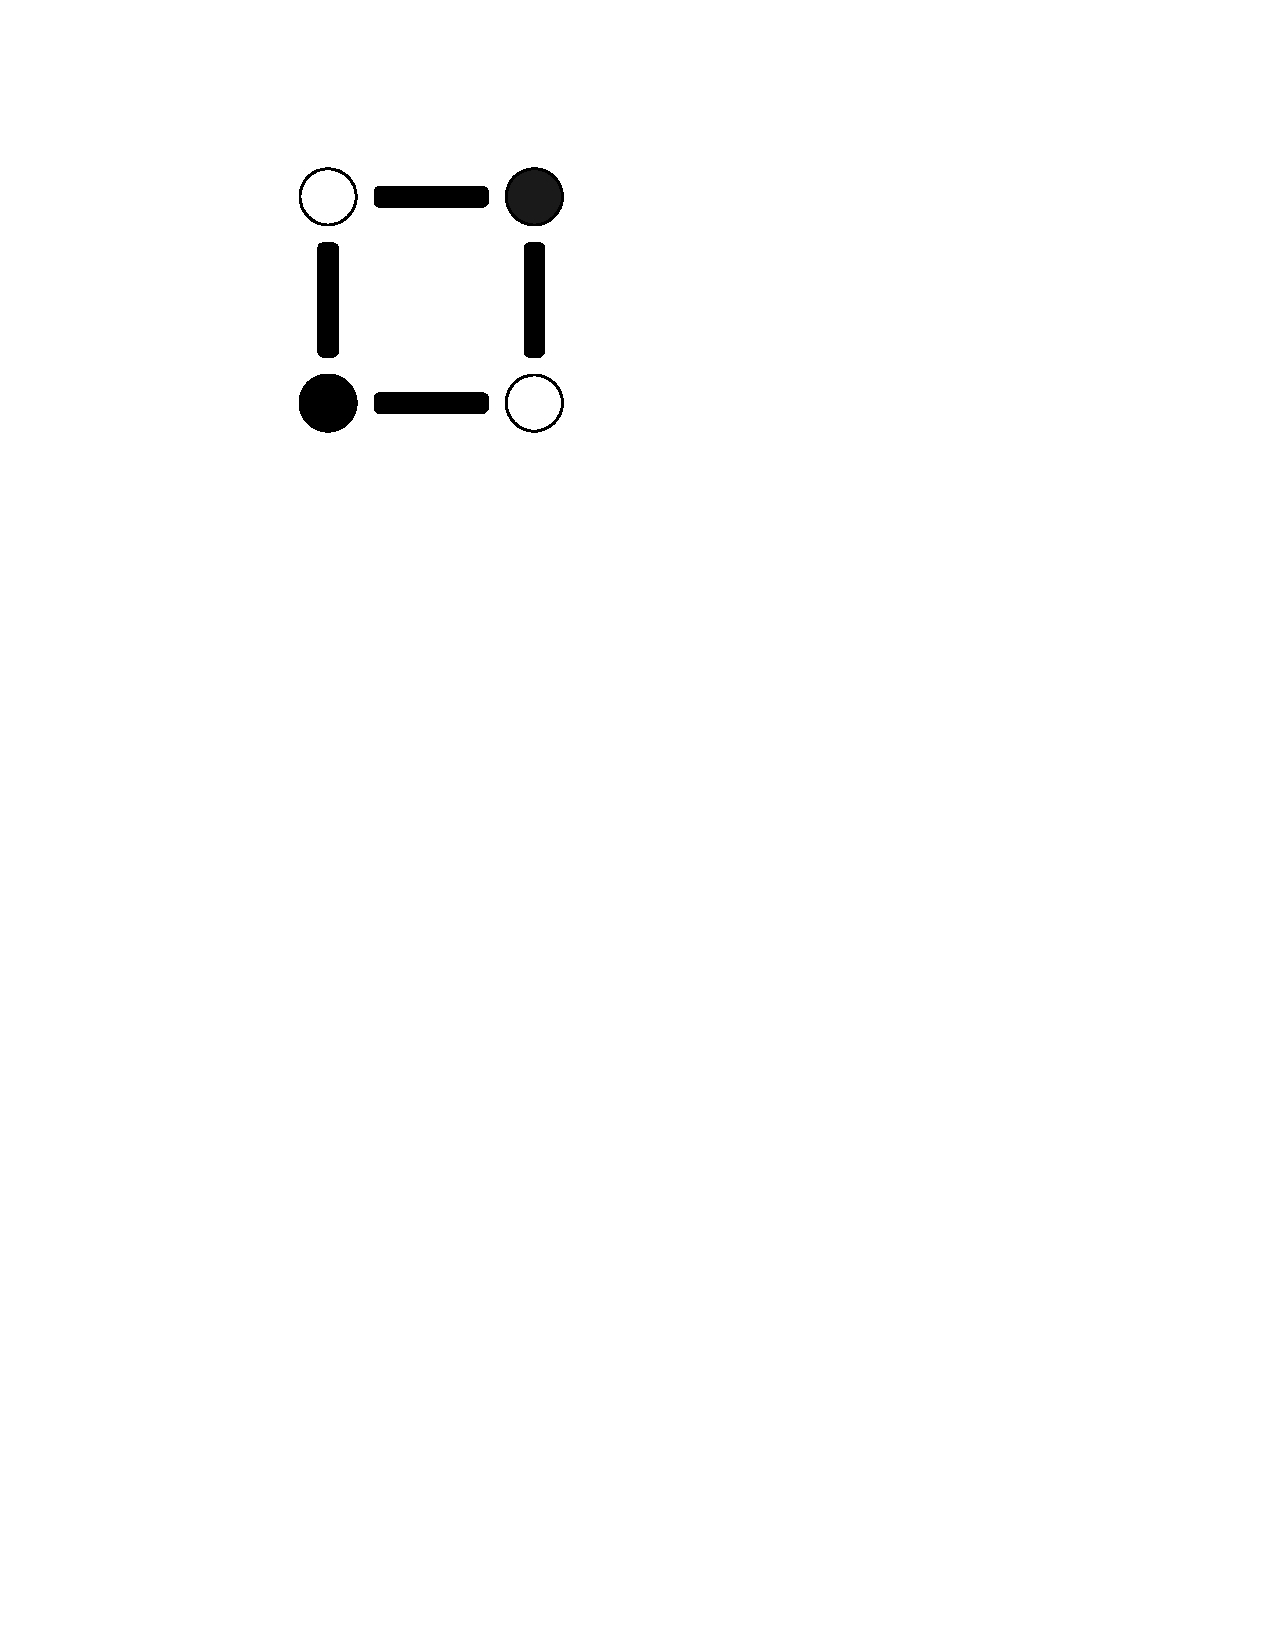
\includegraphics[width=.2\linewidth]{negative.pdf}\label{fig:negative}}
\caption{Positive and negative rectangle contraints. White corresponds to points being added, and black corresponds to the points being subtracted}
\label{fig:rectangles}
\end{figure}

With this, we have simplified our constraints significantly and only lost an $O(1)$ factor to the optimum.

\section{Possible Approaches}

\subsection{Experiments}

We ran experiments to see how the integer linear program compared to the linear program. In particular, we wanted to see whether they were the same, or what the integrality gap was. We wrote a program in python that would generate instances of the points in the plane problem and tried to solve it with the second linear program. We used a python library PuLP which in turn used GLPK (GNU Linear Programming Kit). We were able to run experiments and showed that in fact there are cases for which the second linear program had an integrality gap strictly greater than 1. In most cases, the integrality gap was between 1 and 2, and never surpassed 1.6.

\subsection{Max Flow}

We tried to solve the integer linear program for an optimal solution. This would have solved the points in the plane problem. We wanted to write the integer linear program as an equivalent flow problem. We were unsuccessful at coming up with such a formulation, and we believe that no simple max flow formulations of this exact LP exist. A natural way of rewriting this problem as a flow problem would probably result in a flow problem with integral capacities and costs, given that all coefficients in the constraints in the linear program are integers. However, the Integral Flow Theorem would then guarantee that the optimal solution to this LP would be integral. This cannot be the case, since experimental evidence shows there is an integrality gap strictly greater than 1.

\subsection{The Dual}

The next thing we wanted to do was take the dual to see if we could derive some combinatorial interpretation that could simplify the problem or even find other potential algorithms for the problem.
Representing the linear program as a matrix, the primal linear program looks like:
\[ \min \hspace{.1in} [ \begin{array}{cccc} 1 & 1 & \dots & 1 \end{array} ] \left[\begin{array}{c} b_{11} \\ b_{12} \\ \vdots \\ b_{nn} \end{array} \right]\]
such that
\[ \left[ \begin{array}{c} \vdots \\ \text{ $P$ = positive rectangles } \\ \vdots \\ \text{ $N$ = negative rectangles } \\ \vdots \\ \text{ $I_n'$ = equality } \end{array} \right] 
\left[\begin{array}{c} b_{11} \\ b_{12} \\ \vdots \\ b_{nn} \end{array} \right] 
\begin{array}{c} \\ \leq \\ \\ \\ \leq \\ \\ \\ = \end{array} 
\left[\begin{array}{c} 1 \\\\ 1 \\\\ \vdots \\\\ 1 \end{array} \right] \]

Where $P$ and $N$ are $\dbinom{n}{2}^2 \times n^2$ matrices, since there are that many positive and negative rectangles. $I_n'$ is the some permutation of identity matrix with extra zero columns. Furthermore, we require that all variables are positive. 

We can compute the dual:
\[ \max y^T \left[ \begin{array}{c} 1 \\ 1 \\ \vdots \\ 1 \end{array} \right] \]
such that
\[ \left[ \begin{array}{ccc} \vdots & \vdots & \vdots \\
					  P^T & N^T & I_n \\
					\vdots & \vdots & \vdots \end{array} \right] y
\leq  \left[ \begin{array}{c} 1 \\ 1 \\ \vdots \\ 1 \end{array} \right] \]
Where the first $n$ variables in $y$ can take on any value, and the rest must all be negative. 

This will corresponds to the following:

We will have a variable for each positive rectangle and each negative rectangle, denoted $b_{ij, lk}$ and a variable for each point that was set $a_{xy}$. Then for each point $xy$, if $xy$ is set, then we have the following constraint:
\[ a_{xy} + \sum_{\begin{array}{c}\text{rectangles where}\\\text{$xy$ on corner}\end{array}} b_{ij, lk} - \sum_{\begin{array}{c}\text{rectangles where}\\\text{$xy$ on side}\end{array}} b_{ij,lk} \leq 1 \]
If $xy$ is not set, then the $a_{xy}$ term is not present. We want to maximize
\[ \sum a_{xy} + \sum b_{ij,lk} \]
where $b_{ij,lk} \leq 0$. The $a$'s are unconstrained. We would like to set the values of the rectangles that have points two points on their corners as negative, since then we could raise $a_{xy}$ by the same amount in both corners and thus increase the objective.

\section{An Unbounded Integrality Gap}

We show that the linear programming relaxation will probably not yield an $O(1)$-approximation.

There are known instances of the problem that require $O(n\log n)$ additional points. On one of these instances, if you set all the neighboring points of set points to $0.5$. To see that this solution is feasible, note that every rectangle created from points of value 1 will be satisfied, since the rectangle must contain at least 2 points of value $0.5$. All the rectangles created by one point of value $1$ and one point of value $0.5$ will be satisfied by a point of value $0.5$ adjacent to the point $1$. Finally each rectangle with opposite corners $0.5$ will automatically be satisfied since the sum of the two is already less than or equal to 1. This feasible solution in has an optimum of size $O(n)$; therefore, the integrality gap is $O(\log n)$. 

Figure~\ref{fig:integralitygap} demonstrates the lower bound of the integrality gap. Figure~\ref{fig:optimum} shows the optimum of the integer linear program, where the white circles are the instance of the problem and the green circles are the variables that are set to 1. It is clear from the picture that all constraints are satisfied and that this is the minimum number of points needed. Figure~\ref{fig:lpsolution} gives a $O(n)$ feasible solution to the linear program where the white circles indicate the instance of the problem and the red circles are the points that are assigned to $0.5$. 

\begin{figure}
\centering
\subfigure[Optimal solution to integer linear program]{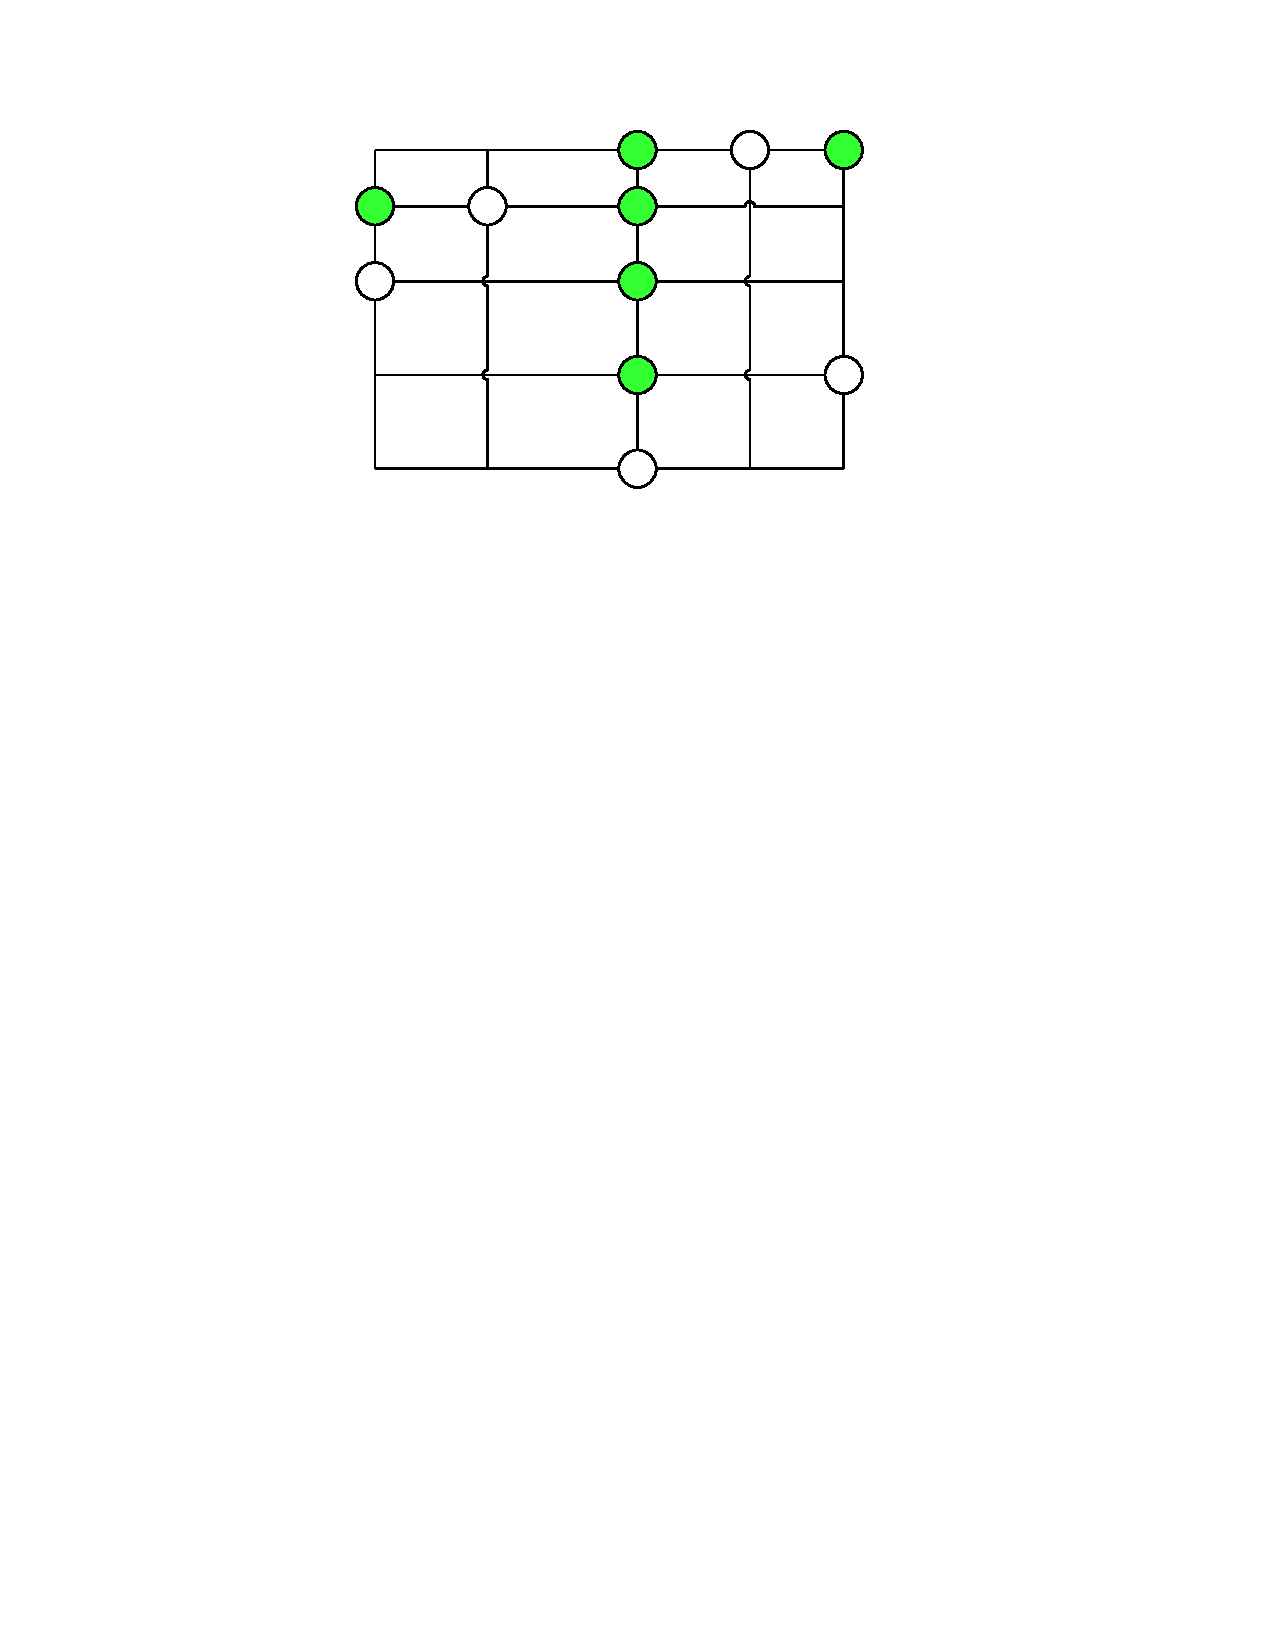
\includegraphics[width=0.4\linewidth]{optimum.pdf}\label{fig:optimum}}
\subfigure[Feasible solution to linear program]{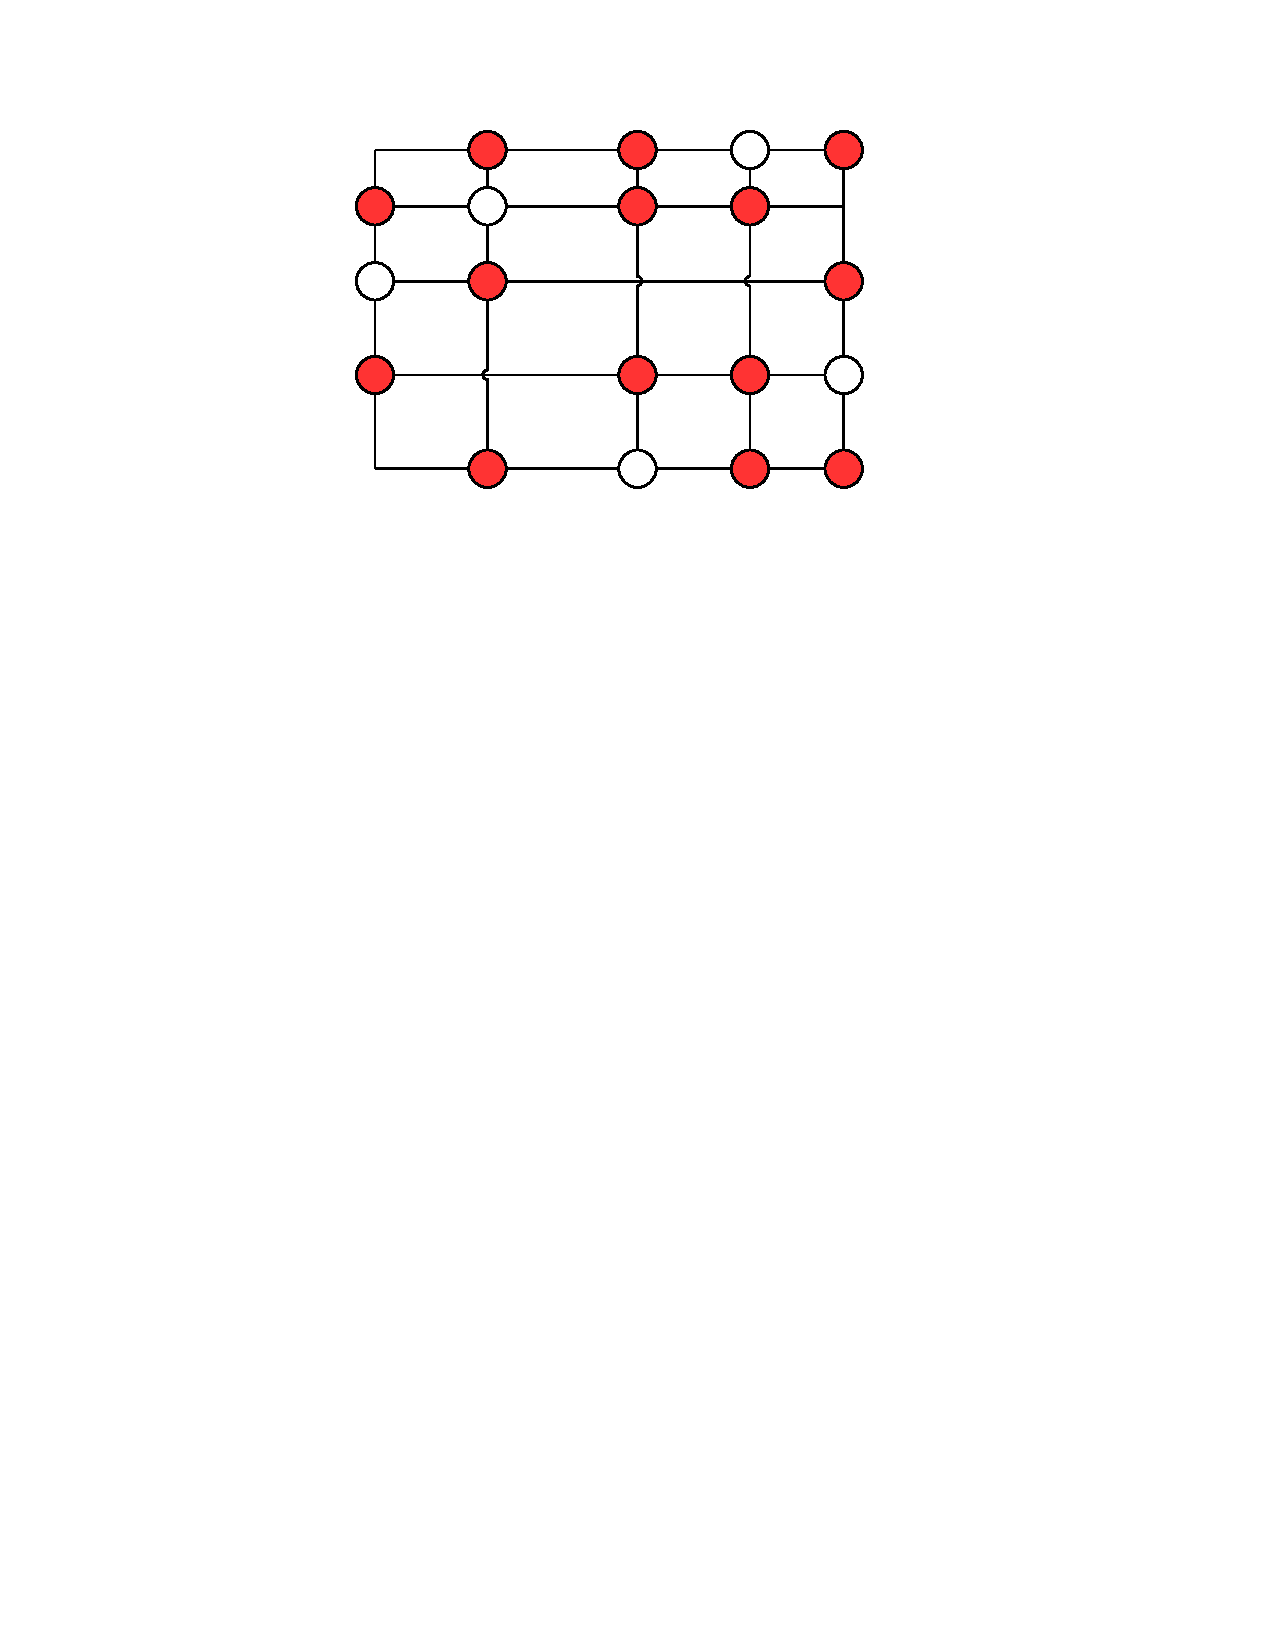
\includegraphics[width=.4\linewidth]{lpsolution.pdf}\label{fig:lpsolution}}
\caption{Integrality gap of linear program}
\label{fig:integralitygap}
\end{figure}

To illustrate how this is a big problem, suppose we had a rounding scheme from the linear programming relaxation. Lets call the rounded solution $R$, $LP$ will be the optimum of the relaxed linear program, and $ILP$ will be the optimum of the integer linear program. What we know is that
\[ LP \leq ILP \leq R \leq O(\log n)LP \]
However, without computing $ILP$, we won't be able to show that $R$ and $ILP$ are close ($O(1)$-factor away). This means that typical rounding scheme proofs won't work. 

\section{Extending the Method}

Our hope is to show that this technique of producing an unbounded integrality gap extends to all linear programming interpretations of arboral satisfaction. However, it seems very difficult to make such claims, and so we have only focused on ``natural" linear programming interpretations.

We make the one assumption that all variables corresponds to points, and that the variable is set to $1$ when the point is included in the set $Q$ and $0$ otherwise. Without loss generality, we can assume that all contraints are either $\leq$ contraints, and there are an additional $n$ contraints to set the variables which corresponds to points in $P$ to $1$. Also, without loss of generality, we can rescale the contraints so that they are all $\leq 1$. 

\begin{observation}
For each two points $x$ and $y$ which form a rectangle, there exists a contraint $C$, such that
\[ C: a_1x + a_2y + \dots \leq 1 \]
where $a_1 \leq 1$, $a_2 \leq 1$ and $a_1 + a_2 > 1$. 
\end{observation}

\begin{proof}
This just follows from the fact that if there is only one point, the set is arborally satisfied. Which means that all positive coefficients are less than $1$. Also since setting points $x$ and $y$ alone is not arborally satisfied, there exists a contraint which is violated.
\end{proof}

\begin{observation}
For each two points $x$ and $y$ which form a rectangle, let $z$ be a different point on a corner of the rectangle spanned by $x$ and $y$, then
\[ C: a_1x + a_2y - a_zz + \dots \leq 1 \]
where $a_1 + a_2 - a_z \leq 1$ and so $a_z < 0$.
\end{observation}

\begin{proof}
This follows from the fact that constraint $C$ was not satisfied without $z$ but it is satisfied with $z = 1$. 
\end{proof}

In fact, we can generalize the statement to all points in the edges.
\begin{observation}
For each two points $x$ and $y$ which form a rectangle, let $z_1$ and $z_2$ be points on the edge of the rectangle across from each other, then
\[ C : a_1x + a_2y + a_{z_1}z_1 + a_{z_2} + \dots \leq 1\]
where $a_1 + a_2 + a_{z_1} + a_{z_2} \leq 1$. 
\end{observation}

\begin{comment}
We make three assumptions about ``natural" linear programs for this problem:

1) Grid points should correspond to variables and vice versa, and variables should be 0 or 1 depending on whether or not the grid point is present.

2) There should be one constraint for each possible grid rectangle. It does not seem like it makes sense for a given rectangle's arboral satisfaction to rely on two or more constraints.

3) The structure of the constraint does not depend on the rectangle that corresponds to it. Essentially, this is just assuming that we can write down all constraints in a general form, as we do with equations (1), (2), (3), and (4).

Whether or not these assumptions are sufficiently general or even reasonable is unclear. However, the two linear programs we have shown clearly meet these assumptions, and we believe there is likely an unbounded integrality gap for all programs that do meet these assumptions.

Consider the constraint corresponding to some given positive rectangle defined by two corner vertices $b_{ij}$ and $b_{kl}$ where $i<k$ and $j< l$. We know what points (in constraint space, not the plane) should satisfy the constraints and what do not, so we can use this information to reveal the structure of the constraint. In particular, if at least one of $b_{ij}$ or $b_{kl}$ is 0, the point (in constraint space) should satisfy the constraint no matter what. However, if both $b_{ij}$ and $b_{kl}$ are 1, then we don't want this to be a satisfying arrangement unless some other $b$ within the rectangle is set to 1. Since we can satisfy the rectangle by including any $b$ in the rectangle, we note that the coefficients of these $b$'s must be the opposite of the coefficients on $b_{ij}$ and $b_{kl}$. WLOG, assume the coefficients on $b_{ij}$ and $b_{mn}$ are positive (otherwise we can just multiply both sides by -1), and this tells us the LHS of the constraint is of the form
\[ w_{ij}b_{ij} + w_{kl}b_{kl} - \sum_{b_{mn} \in \text{rectangle}} w_{mn}b_{mn} \]

If no points in the plane are present, the constraints should all be satisfied. We consider the following idea:

For each point $b_{ij}$ in the given point set $P$, increase $b_{i+1,j}$ by $w_{i,j}/w_{i+1,j}$, and increase $b_{i-1,j}$ by $w_{i,j}/w_{i-1,j}$. We can easily check that this leads every LHS of every constraint corresponding to a rectangle formed by two points in $P$ to equal 0. If we could guarantee this for all rectangles, then we would be finished.
\end{comment}

\section{Conclusions}

Our results have shown that the natural linear programming interpretations of the points in the plane do not seem to be particularly helpful in solving the problem. Standard ways of tackling linear programs such as looking at their duals or trying to transform them into max flow problems are not useful for the linear programs we were able to write down.

We were able to show an unbounded integrality gap, and we hope that we can show an unbounded gap for all linear programs.

\bibliography{references}
\bibliographystyle{plain}

\end{document}
